\chapter{Optimierung der Simulation}
\label{ch:opt}
In der vorangegangen Kapiteln wurde die Umsetzung der Simulation erläutert und gezeigt, dass ein funktionsfähiges Framework validiert werden konnte. Im letzten Schritt dieser Ausarbeitung geht es um die Performance Optimierung hinsichtlich der Rechenzeit. Somit soll die Effizienz gesteigert und Schwachstellen im Code korrigiert werden. An dieser Stelle werden die Randbedingungen kurz erläutert, um gleiche Testbedingungen zu garantieren und um die Ressourcen des Rechners vollständig auszunutzen:
\begin{itemize}
	\item Um statistisch aussagekräftige Ergebnisse bezüglich der Rechenzeit zu erhalten werden 5 Läufe durchgeführt und am Schluss gemittelt.
	\item Hintergrundprozesse sollen vermieden werden.
	\item Der Rechner (Laptop) soll an einer Stromquelle angeschlossen sein. 
\end{itemize}
\section{Profiling}
Mithilfe des in Visual Studio integrierten Leistungsprofilers  wird das Laufzeitverhalten der Simulation untersucht. Somit sollen Problembereiche aufgezeigt werden, die kritisch hinsichtlich der Rechenzeit sind. In dieser Arbeit wird der Profiler genutzt, um die Anzahl der Aufrufe und Durchläufe von Funktionen festzustellen. Somit kann das Hauptaugenmerk auf Funktionen gerichtet werden, die durch ihre Aufrufe viel Zeit in Anspruch nehmen. In Tabelle \ref{tab:.profiler} werden besagte Funktionen mit ihrer jeweiligen CPU-Zeit aufgelistet. 
\begin{table}[h]
	\centering\begin{tabular}{llp{5cm}l}
	\textbf{Nr.} &	\textbf{Methode} & \textbf{Kurzbeschreibung} &\textbf{CPU-Zeit}\\
	1&	Trajectory6Dof::log6DofData() & Daten-Logging der einzelnen Module&50,79\% \\
	2&	updateAutopilot::updateStateController(...) & Zustandsregler & 22,62\% \\
	3&	LinearInterpolation::linearInterpolation2D(...) & Tabellen-Interpolation & 13,18\%
	\end{tabular}
\caption{Ergebnisse des Leistungsprofilers}
\label{tab:.profiler}
\end{table}\noindent\\
Es ist offensichtlich, dass das Erzeugen der Output-File den größten Einfluss auf die Gesamtrechenzeit hat. Im nächsten Schritt müssen mögliche Ursachen gefunden werden, die für die jeweiligen Funktionen die Rechenzeit beeinflussen. Im Anschluss muss eine Lösung für die Rechenzeit-Reduktion gefunden werden. In Tabelle \ref{tab:korrektur} werden die möglichen Ursachen und Lösungsansätze gegenüber gestellt.
\begin{table}[h]
	\centering\begin{tabular}{lp{6cm}p{4cm}}
		\textbf{Nr.} & \textbf{Ursachen} & \textbf{Lösungsansatz}\\
		1 & -nicht benötigte Daten werden geloggt & -Reduktion des Outputs \\
									  & -std::to\_string (25,5\%) & -alternative Methode finden (Benchmarking)\\
									  &&\\
		2 & Eigen::Library & alternative Bibliotheken \\	
									  &&\\
		3	& Index suche im Array & 	Suchmethoden anpassen		
	\end{tabular}
	\caption{Gegenüberstellung Ursachen und Lösungsansätze der Rechenzeit}
	\label{tab:korrektur}
\end{table}
\section{Code Optimierung}
Wie in Tabelle \ref{tab:korrektur} beschrieben, wurde unter Punkt 1 der Output der einzelnen Module reduziert. Zusätzlich wird im nächsten Abschnitt nach Alternativen für die \textit{std::to\_string} Methode gesucht. Da das Hauptaugenmerk auf der Überprüfung der Flugregelung steht, wurden Parameter vernachlässigt, die wenig Aussagekraft darüber besitzen.\\ Der Flugzustandsregler (Punkt 2) selbst beruht in großen Teilen auf linearer Algebra. In dieser Ausarbeitung wurde die lineare Algebra durch die Open Source Bibliothek \textit{eigen} realisiert. Eine Effizienzsteigerung wäre mithilfe einer alternativen Bibliothek denkbar, wurde aber nicht weiter betrachtet. Der Aufwand, sämtliche mathematischen Operationen in der Gesamtsimulation abzuändern wäre zu groß. Nach \cite{TuxFamily.2018} gibt es spezielle Einstellungen für Visual Studio, um die Performance der Bibliothek zu steigern, welche letztlich umgesetzt wurden. \\  Für die Interpolation (Punkt 3) werden Stützstellen benötigt. Diese Stützstellen zu finden ist mit großem Aufwand verbunden, da dass gesamte Array durchsucht werden muss. Es wurde versucht, diese Suche zu beschleunigen. Diese algorithmische Optimierung hat sich als äußerst komplex rausgestellt und konnte nicht gelöst werden. Das Ergebnis des ersten Teils der Optimierung ist in Abbildung \ref{fig:opt1} zu sehen.\newpage
\begin{figure}[h]
	\centering
	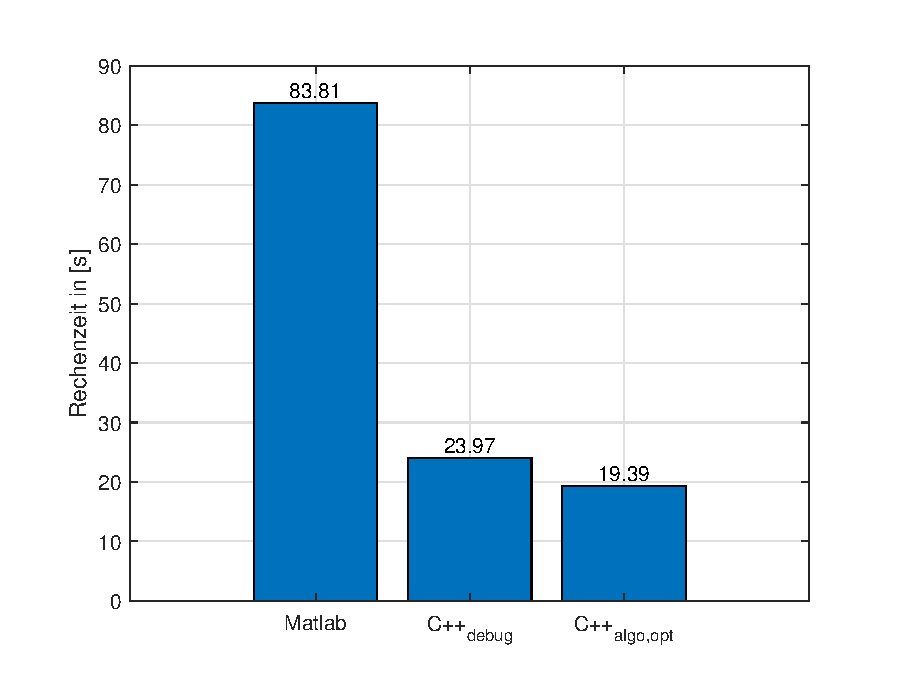
\includegraphics[width=0.6\linewidth]{opt1}
	\caption{Gegenüberstellung nach Code Optimierung Teil 1}
	\label{fig:opt1}
\end{figure}\noindent
Durch kleinere Maßnahmen im Code konnte die Rechenzeit nochmals um rund 4 Sekunden reduziert werden, was in etwa 19\% zum ursprünglichen C++ Code und 76,86\% zu Matlab schneller ist.
\subsection{Benchmarking String-Typumwandlung}
\label{sec:bench}
Wie in Tabelle \ref{tab:korrektur} angedeutet, beschäftigt sich dieser Abschnitt mit der Untersuchung von verschiedenen Möglichkeiten, die Typumwandlung in \textit{Strings} umzusetzen. Neben den Standardbibliotheken werden an dieser Stelle auch Open Source Bibliotheken hinzugezogen. Zum Einen wurden zwei Methoden der Boost-Bibliothek \cite{C++StandardsCommittees.2018} genutzt. Besagte Bibliothek wurde zur Produktivitätssteigerung in C++ erschaffen. Zum Anderen wurde die C++ String Toolkit Library (StrTk) von \cite{Partow.2018} genutzt. Dabei handelt es sich um eine Bibliothek, die speziell für den Umgang von Strings implementiert wurde. In Tabelle \ref{tab:benchmarking} werden die unterschiedlichen Methoden aufgelistet. 
\begin{table}[h]
	\centering\begin{tabular}{l}
		\textbf{Methode}  \\
			std::ostringstream \\
			sprintf\_s \\
			std::to\_string\\
			boost::lexical\_cast<std::string>(...)\\
			boost::str(boost::format("\%.4f") \% (value))\\
			strtk::type\_to\_string<double>(value)
			\end{tabular}
	\caption{Methoden für die Typumwandlung in \textit{String}}
\label{tab:benchmarking}
\end{table}\newpage
Das Ergebnis des Benchmarkings ist in Abbildung \ref{fig:benchmarking} zu sehen. In diesem Fall erwies sich die Methode sprintf\_s als sehr effizient.\\
\begin{figure}[h]
	\centering
	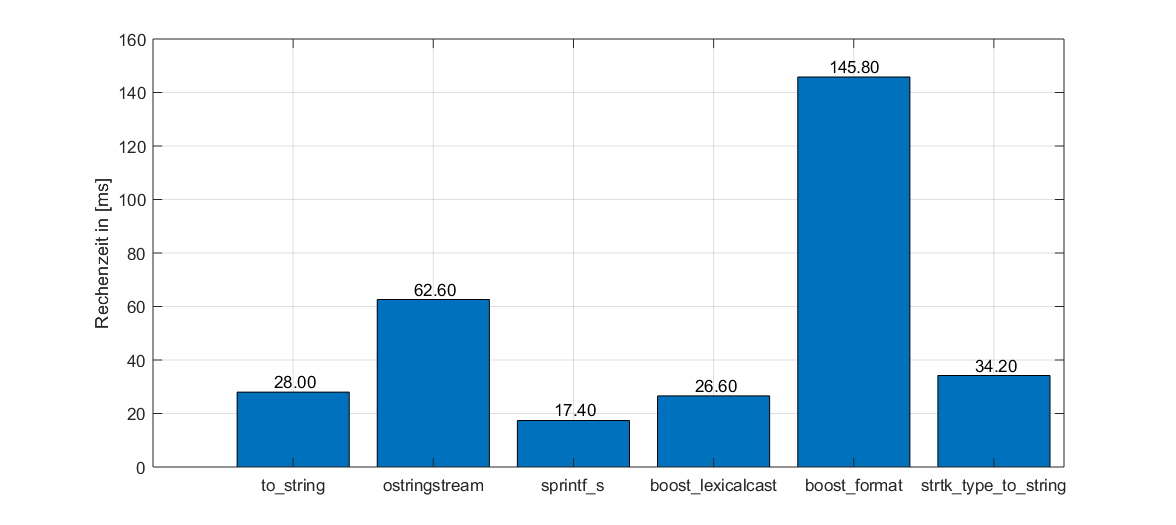
\includegraphics[width=0.8\linewidth]{benchmarking}
	\caption{Ergebnisse des Benchmarkings}
	\label{fig:benchmarking}
\end{figure}\noindent\\
 Die Methoden der Open Source Bibliotheken enttäuschen hingegen und werden aus diesem Grund in dieser Arbeit nicht weiter betrachtet. Aufgrund des Benchmarking-Ergebnisses wurde die std::to\_string Methode durch sprintf\_s ersetzt. Das Ergebnis der zweiten Code Optimierung ist in Abbildung \ref{fig:opt2} zu sehen.\\
\begin{figure}[h]
	\centering
	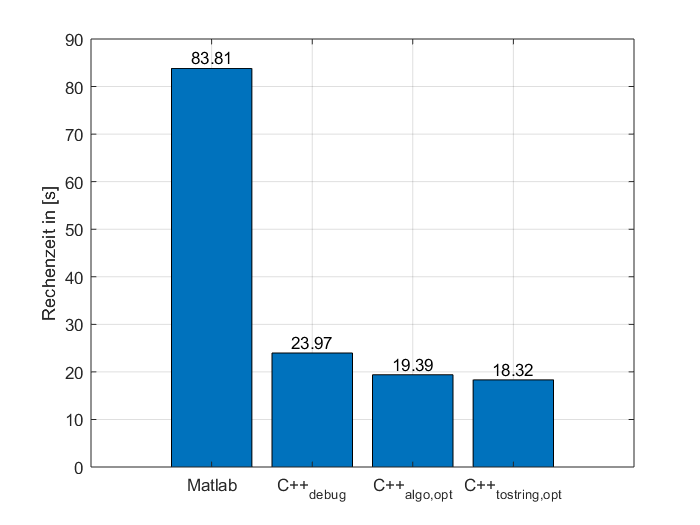
\includegraphics[width=0.6\linewidth]{opt2}
	\caption{Gegenüberstellung nach Code Optimierung Teil 2}
	\label{fig:opt2}
\end{figure}\noindent\\
Auch wenn die Rechenzeit sich nur minimal verbessert hat, so ist dies dennoch als gutes Ergebnis zu betrachten. Quantitativ ausgedrückt, hat sich die Rechenzeit gegenüber der ersten Optimierung konnten nochmals 5,5\% verbessert. Stand hier wurde die Rechenzeit gegenüber Matlab um 78,1\% verbessert.
\section{Parallelisierung und Vektorisierung}
Eine weitere Möglichkeit, neben der Code Optimierung, die Performance zu steigern ist die Zuhilfenahme von automatischer und gesteuerter Parallelisierung \cite{Kessler.Wintersemester201718}. Zusätzlich wurde auch noch der Einfluss von automatischer Vektorisierung untersucht. Die Ergebnisse der Parallelisierung sind auf den jeweiligen Rechner bezogen, wo diese durchgeführt wurde. Aus diesem Grund wird an dieser Stelle der Rechner, womit die Implementierung durchgeführt wurde, kurz aufgezeigt. Die grundlegenden Daten des Rechners sind in Tabelle \ref{tab:Rechnerdaten} zusammengefasst.
\begin{table}[h]
	\centering	\begin{tabular}{l p{10cm}}
		\textbf{Eigenschaft} & \textbf{Beschreibung/Wert}\\
		Betriebssystem & Windows 10\\
		Prozessor & Intel(R) Core(TM) i7-6600U CPU @ 2.60GHz 2.81GHz\\
		RAM & 8 GB\\
		Systemtyp & 64-Bit 
	\end{tabular}
	\caption{Rechnerdaten}
	\label{tab:Rechnerdaten}
\end{table}\\
Ausgangslage für die weitere Optimierung stellt das Ergebnis der  zweiten Code Optimierung aus Abschnitt \ref{sec:bench}.
\subsection{Automatische Parallelisierung und Vektorisierung}
Die automatische Parallelisierung und Vektorisierung kann schnell und einfach über Compiler-Flags durchgeführt werden. Der Compiler entscheidet selbstständig, ob er beispielsweise einen Abschnitt parallelisiert oder nicht. Die in dieser Arbeit genutzten Flags von Visual Studio werden in Tabelle \ref{tab:compilerflags} aufgezeigt. 
\begin{table}[h]
\centering	\begin{tabular}{ll}
		\textbf{Flag-Name} & \textbf{Verwendung}\\
		Qpar & automatische Parallelisierung\\
		arch & automatische Vektorisierung
	\end{tabular}
\caption{Compiler-Flags für automatische Parallelisierung und Vektorisierung}
\label{tab:compilerflags}
\end{table}\noindent\\
Die Flags werden sowohl einzeln als auch gemeinsam betrachtet. In Abbildung \ref{fig:compilerflags} sind die Ergebnisse dargestellt.\newpage
\begin{figure}[h]
	\centering
	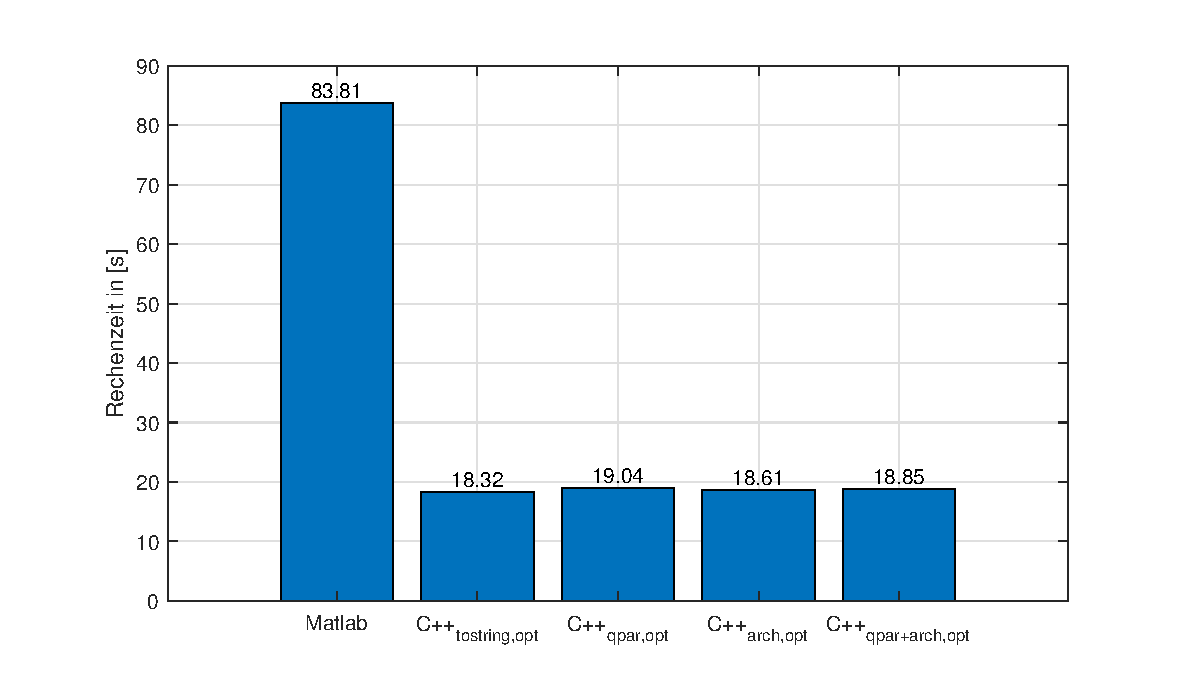
\includegraphics[width=0.7\linewidth]{compilerflags}
	\caption{Ergebnisse der automatischen Parallelisierung und Vektorisierung}
	\label{fig:compilerflags}
\end{figure}\noindent\\
Durch die automatische Parallelisierung und Vektorisierung wurde die Performance geringfügig schlechter. Dieses Ergebnis ist nach \cite{Kessler.Wintersemester201718} durchaus möglich. Aufgrund des fehlenden Performance-Gewinn, wird auf die Flags im Weiteren verzichtet. 
\subsection{Gesteuerte Parallelisierung}
Bei der gesteuerten Parallelisierung wird der Compiler durch Direktiven im Code angewiesen eine Parallelisierung durchzuführen. In dieser Ausarbeitung wurde der OpenMP Standard genutzt.\\
Es war leider nicht möglich, ein sinnvolles Ergebnis zu erzeugen. Grund hierfür liegt im Ablauf der Simulation selbst. Die Berechnung der Trajektorie findet lediglich in einer for-Schleife statt. Somit sind die Ergebnisse der direkt aufeinanderfolgenden Zeitschritte abhängig voneinander. Aus rein physikalischer Sicht ist es beispielsweise nicht möglich, dass ein Thread schon den nächsten Zeitschritt berechnet, bevor der vorangegangene Zeitschritt berechnet wurde. Somit wird auch die gesteuerte Parallelsierung nicht weiter betrachtet.\\

